% RESULTADOS-------------------------------------------------------------------

\chapter{Análise e Discussão dos Resultados}
\label{chap:resultados}

Este capítulo discute os resultados obtidos nas duas etapas do experimento definidas no Capítulo~\ref{chap:metodologia}: treinamento e teste.

\section{Robustez}
\section{Unicidade}

% ------------------------- Treinamento
\begin{figure}[h]
	\centering
	\label{fig:limiares-framediff}
	\caption{Teste de limiares para a assinatura framediff}
	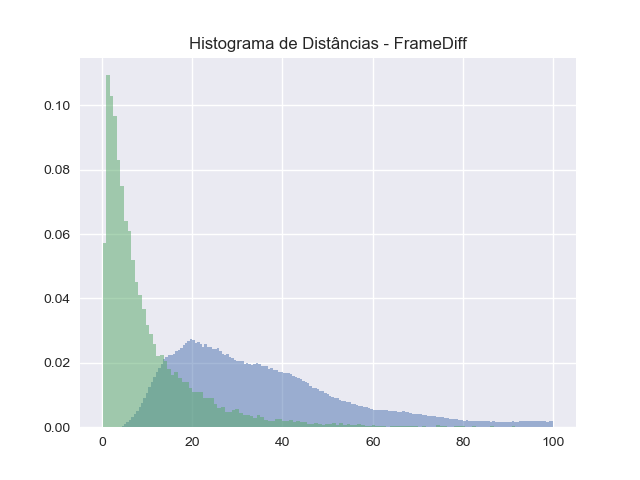
\includegraphics[width=0.8\textwidth]{dados/figuras/experimentos/histograma_FrameDiff.png}
\end{figure}
\begin{figure}[h]
	\centering
	\label{fig:limiares-medidaordinal}
	\caption{Teste de limiares para a assinatura medida ordinal}
	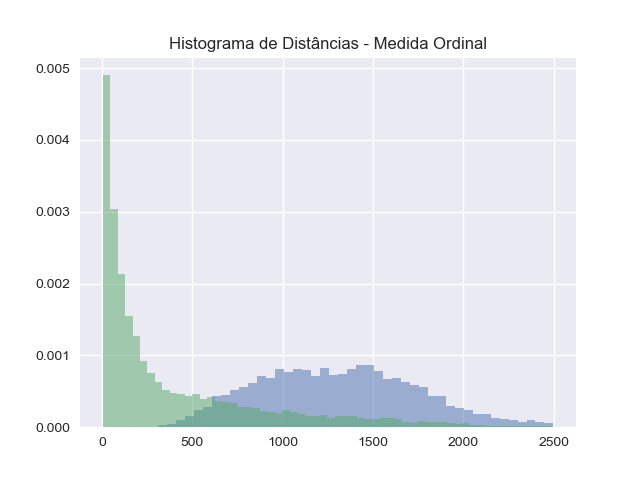
\includegraphics[width=0.8\textwidth]{dados/figuras/experimentos/histograma_Medida_Ordinal.png}
\end{figure}
\begin{figure}[h]
	\centering
	\label{fig:limiares-sceneframe}
	\caption{Teste de limiares para a assinatura sceneframe}
	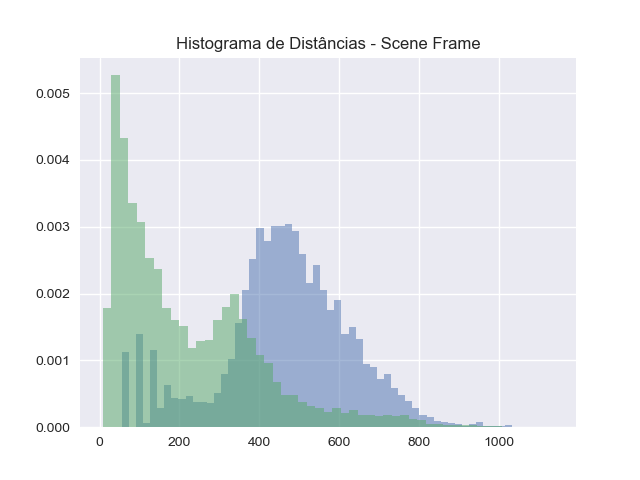
\includegraphics[width=0.8\textwidth]{dados/figuras/experimentos/histograma_Scene_Frame.png}
\end{figure}
\begin{figure}[h]
	\centering
	\label{fig:limiares-gradiente}
	\caption{Teste de limiares para a assinatura gradiente}
	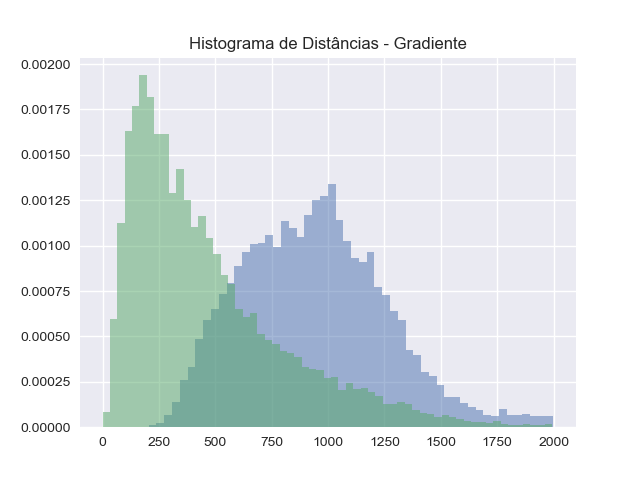
\includegraphics[width=0.8\textwidth]{dados/figuras/experimentos/histograma_Gradiente.png}
\end{figure}
\begin{figure}[h]
	\centering
	\label{fig:limiares-rbp}
	\caption{Teste de limiares para a assinatura rbp}
	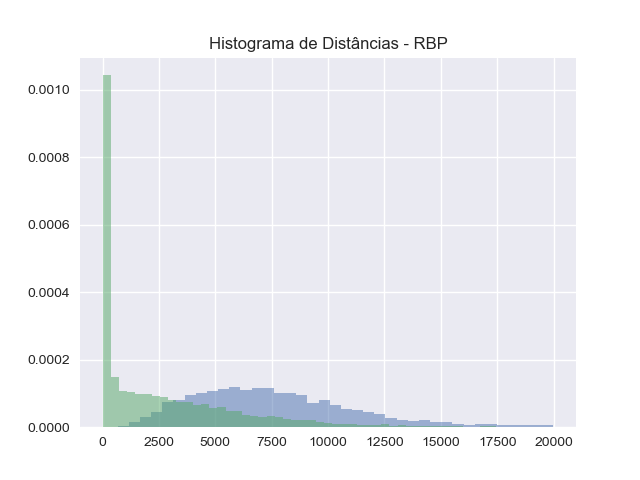
\includegraphics[width=0.8\textwidth]{dados/figuras/experimentos/histograma_RBP.png}
\end{figure}
\begin{figure}[h]
	\centering
	\label{fig:limiares-wavelets}
	\caption{Teste de limiares para a assinatura wavelets}
	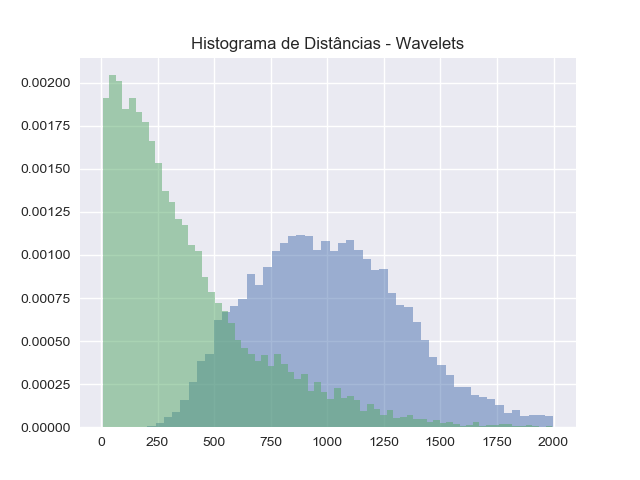
\includegraphics[width=0.8\textwidth]{dados/figuras/experimentos/histograma_Wavelets.png}
\end{figure}

\begin{figure}[h]
	\centering
	\label{fig:limiares-camera-motion}
	\caption{Teste de limiares para a assinatura camera motion}
	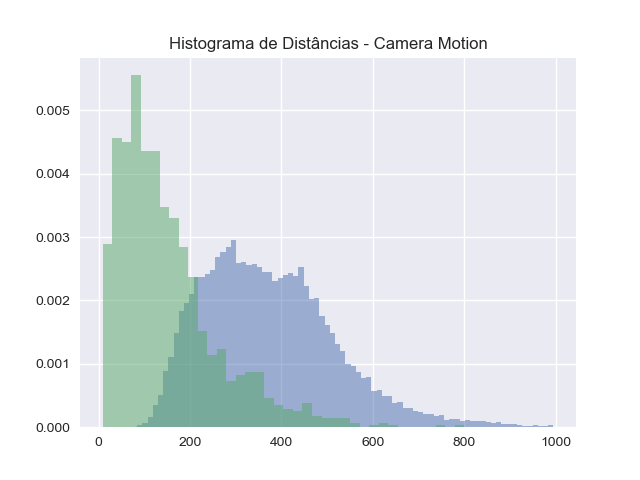
\includegraphics[width=0.8\textwidth]{dados/figuras/experimentos/histograma_Camera_Motion.png}
\end{figure}

\begin{figure}[h]
	\centering
	\label{fig:limiares}
	\caption{Limiares}
	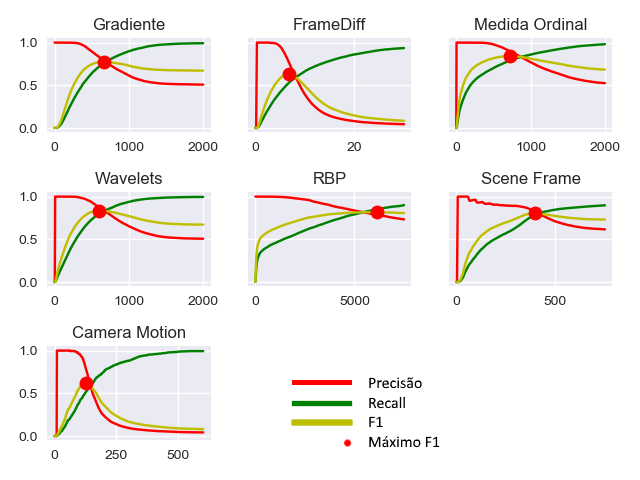
\includegraphics[width=\textwidth]{dados/figuras/experimentos/todos_final.png}
\end{figure}

\begin{table}[h]
	\label{tab:limiares}
	\caption{Limiares por algoritmo por cenário de teste}
	\begin{tabular}{|l|l|l|l|l|l|l|}
		\hline
		\textbf{Assinatura} & \textbf{T.1} & \textbf{T.2} & \textbf{T.3} & \textbf{T.4} & \textbf{T.5} & \textbf{Limiar Final}\\ \hline
		Gradiente & 761.52 & 637.27 & 681.36 & 705.41 & 629.25 & 682.96\\ \hline
		FrameDiff & 6.63 & 6.48 & 6.33 & 6.78 & 6.93 & 6.63\\ \hline
		Medida Ordinal & 657.31 & 729.45 & 661.32 & 725.45 & 749.49 & 704.60\\ \hline
		Wavelets & 597.19 & 593.18 & 625.25 & 601.20 & 625.25 & 608.41\\ \hline
		RBP & 5501.00 & 6793.58 & 6553.10 & 6147.29 & 4569.13 & 5912.82\\ \hline
		Scene Frame & 399.49 & 391.95 & 399.49 & 391.95 & 399.49 & 396.48\\ \hline
		Camera Motion & 111.82 & 123.84 & 107.01 & 139.47 & 128.65 & 122.16\\ \hline
	\end{tabular}
\end{table}


\begin{figure}[h]
	\centering
	\label{fig:final_heatmap}
	\caption{Final}
	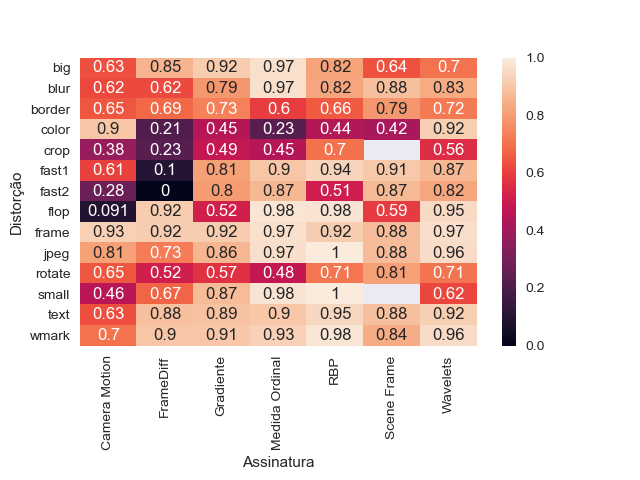
\includegraphics[width=\textwidth]{dados/figuras/experimentos/heatmap_final.png}
\end{figure}